
\section{Data reduction with EDPS: The EDPS Graphic User Interface}
\label{sec:edps_reduction}

In this Section we guide the user to the reduction of science data with an EDPS workflow, exploiting the Graphic User Interface. As example, we refer mostly to the ESPRESSO workflow. 
We assume that EDPS and its components ({\tt edps-gui} and {\tt adari}), the ESPRESSO pipeline with {\tt esorex} and the workflow has been successfully installed and configured in your system (see Section \ref{sec:edps_installation}), the {\tt esorex} is in the system path. If the installation was done via Python virtual environment, then it needs to be activated as described in Section~\ref{sec:edps_installation_procedure}:
\begin{verbatim}
  . <path_to_environment>/edps/bin/activate
\end{verbatim}

We provide examples for other instrument workflows whenever needed to describe features that might not be available in the ESPRESSO workflow.


The most convenient way to reduce data is through the Graphic User Interface (GUI). To launch it, type on a terminal the command:
\begin{verbatim}
    edps-gui
\end{verbatim}
The browser will load the GUI, as shown in Figure \ref{fig:gui}

\begin{figure}
    \centering
    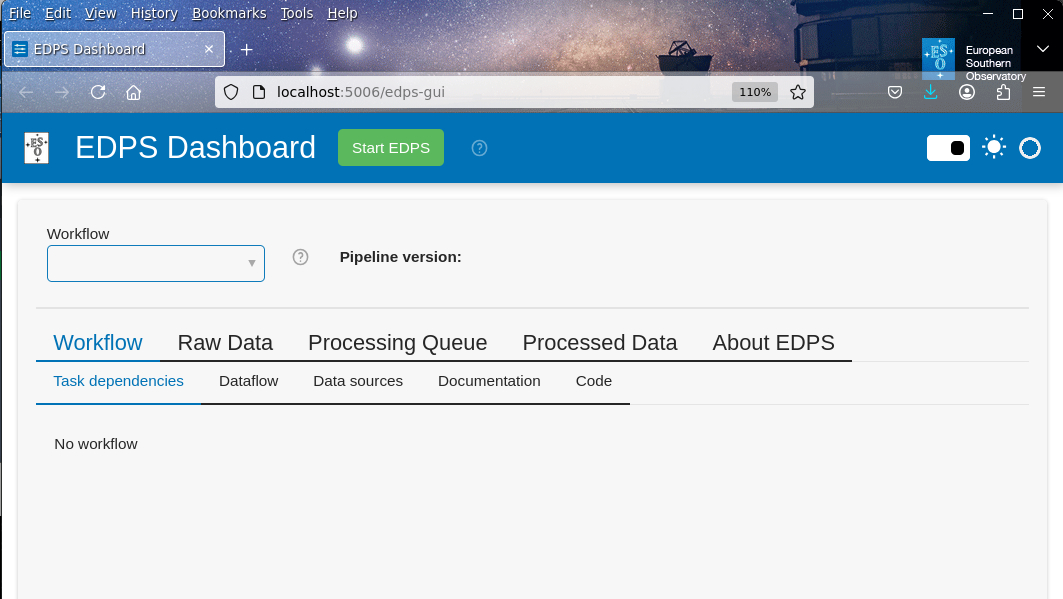
\includegraphics[width=0.95\linewidth]{figures/gui.jpg}
    \caption{The EDPS Dashboard (Graphic User Interface).}
    \label{fig:gui}
\end{figure}

There are few steps to follow to reduce a dataset:

\begin{enumerate}
    \item Load the desired instrument workflow (see \ref{sec:load-wkf}
    \item Specify the input data and create the datasets (see \ref{sec:load-input}
    \item Configure the data reduction strategy, e.g. which datasets to reduce, the steps to execute, the recipe parameters to use, and start the reduction (see \ref{sec:setup}).
    \end{enumerate}

\subsection{Select the workflow} \label{sec:load-wkf}


To start any work with EDPS, you first have to start it by pressing the green button "Start EDPS" at the top of the GUI. The server will read the available workflows and display the first in line. Select the desired workflow (e.g., espresso.espresso\_wkf) from the scroll bar menu "Workflow". A graphic representation of the workflow will be visible in the center of the GUI (see figure \ref{fig:gui-espresso}. Adjust the zoom and the figure width and heigh using the appropriate cursors in the gui

\begin{figure}
    \centering
    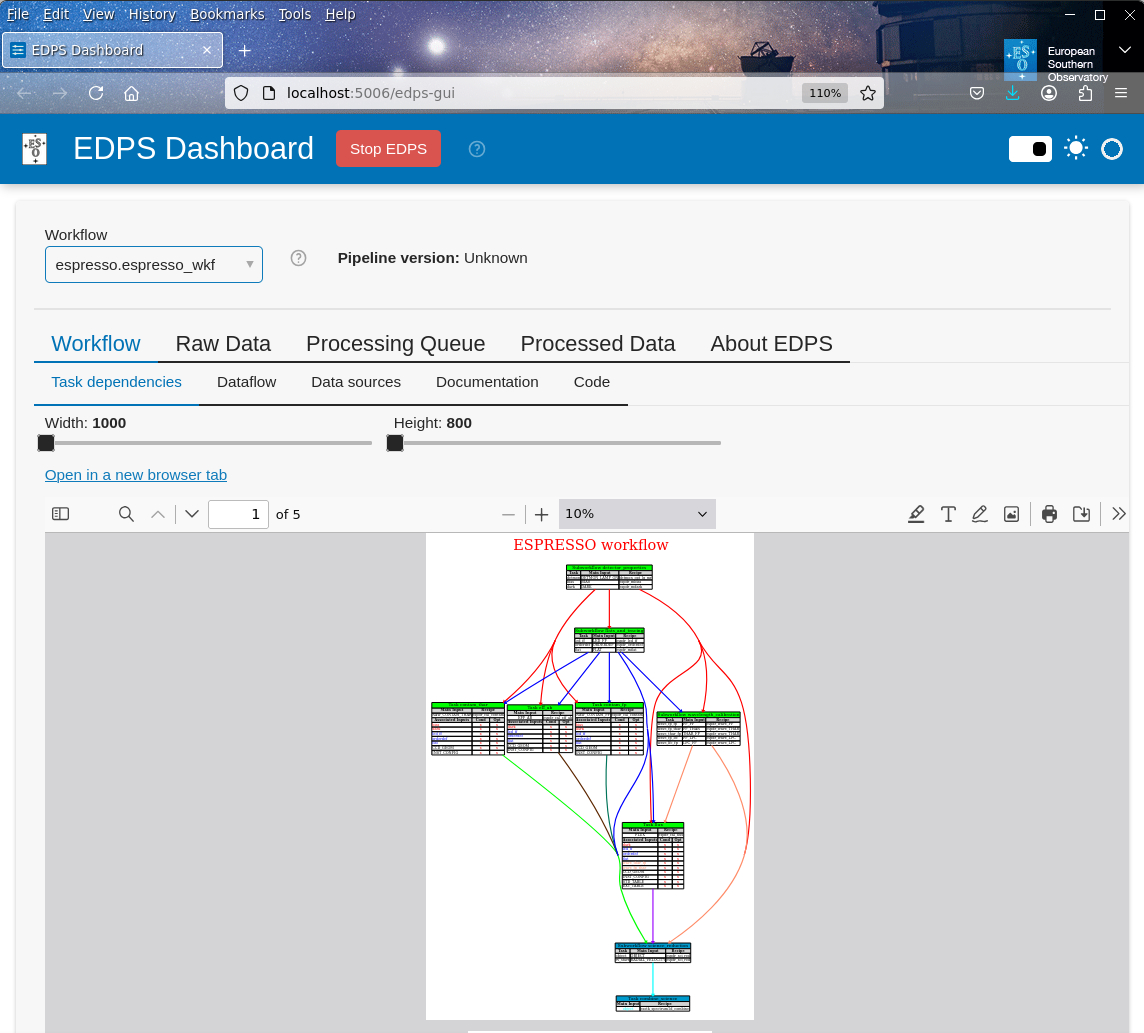
\includegraphics[width=0.95\linewidth]{figures/gui-espresso.jpg}
    \caption{The EDPS GUI with the espresso workflow loaded.}
    \label{fig:gui-espresso}
\end{figure}
\subsection{Select the input data}\label{sec:load-input}
\subsection{Customize the reduction}\label{sec:setup}

\subsection{My first data reduction}\label{sec:myfirst}

A simple reduction of all of the ESPRESSO data in a directory  {\tt input\_directory} can be achieved with a single line command:

 \begin{verbatim}
  edps -w espresso.espresso_wkf 
       -i <input_directory> -o <output_directory>
 \end{verbatim} 

For example, the default location of ESPRESSO demo data when installing the ESPRESSO pipeline with RPMs is {\tt /usr/share/esopipes/datademo/espdr}. EDPS scans the input directory recursively, i.e. the directory and all sub-directories are scanned for data. In addition, the static calibration directory delivered with the pipeline is used. Any FITS file found is classified, the science files are identified, and the best calibrations to be used are associated. All  science exposures with a complete set of calibrations are then processed, and the final data products are copied in the {\tt output\_directory} (if specified). Intermediate files, calibration results, logs and book-keeping information are saved in the general EDPS directory specified during installation (see Section \ref{sec:edps_configuration}).

It is recommended to try this command on the demo data provided with the pipeline. 


\subsection{Closing EDPS}
\label{sec:edps_close}

After the  completion of the first {\tt edps} (section~\ref{sec:myfirst}) command, subsequent calls will start processing with reduced overhead. The reason for this is that EDPS starts a server component that is persistent and remains running in the background even when the processing is completed. Subsequent {\tt edps} commands connect to this server. This mechanism improves the efficiency of the processing. Once no further processing is desired, this server can be closed with the following command:

\begin{verbatim}
    edps -shutdown
\end{verbatim}

One can also pass the option {\tt -shutdown} at every command to close the server after the command execution.




\subsection{Workflows for different pipelines}
 
Depending on the instrument, the workflow reduces science data in different ways. The workflows are similar to the ones documented in detail in the EsoReflex tutorials for each pipeline, which are available at {\url{http://eso.org/pipelines/ }}. Section~\ref{sec:edps_graphic} describes how  to visualise the individual steps of the actually implemented EDPS workflows.

In the cases of ESPRESSO and UVES, individual science observations are processed but not combined. In the case of KMOS, the EDPS worflow first reduces and combines together all the science data that belongs to the same Observing Block, then it combines the results that refer to the same target name and instrument setup. In the case of MUSE, the EDPS workflow first reduces exposures separately and then it combines them according to preference expressed by the user: data from the same Observing Block, or data of the same target name, or data that fall within a certain distance  on  the sky (default).
%(identified by the header keyword {\tt HIERARCH ESO OBS TARG NAME}) and instrument setup (identified by the header keywords {\tt HIERARCH ESO INS GRAT1 NAME}, {\tt HIERARCH ESO INS GRAT2 NAME}, and {\tt HIERARCH ESO INS GRAT3 NAME}).

EDPS processes the data following a default reduction strategy and using certain values for the recipe parameters (whose defaults can vary depending on the type of input data). It is possible to customise the data reduction strategy by changing the values of the recipe parameters, and eventually by activating or de-activating some reduction steps according to the science needs. All these options are instrument-dependent, see Section \ref{sec:edps_parameters} for further details.


\subsection{Location of reduced data and quality control plots.}
\label{sec:edps_output_dir}

%The {\tt <output\_directory>} is the directory where the final products of the final reduction steps are saved (see Sections \ref{sec:edps_output_dir} and \ref{sec:edps_output_dir_2}). If the directory does not exist, it will be created. 

EDPS saves the products into two directories. The first contains all recipe  products, logs and plots (Section \ref{sec:edps_output_dir_1}), whereas the second one, which is optional, contains only the results of the last reduction steps (Section \ref{sec:edps_output_dir_2}).

\subsubsection{Reduced data, logs, quality plots and book-keeping}
\label{sec:edps_output_dir_1}
All recipe products, including all logs, book-keeping and intermediate files are saved into the directory specified in Section \ref{sec:edps_configuration} (default: {\tt \textasciitilde/EDPS\_data)}. This directory should not be deleted, even after the execution of EDPS. It is used for bookkeeping purposes. EDPS will use the files stored there to run efficiently. Among other things, EDPS will reuse products from that directory instead of re-executing a recipe whenever possible ("smart re-run").  The location of this directory can be changed by changing
the value of {\tt base\_dir} parameter in the configuration file {\tt \textasciitilde/.edps/application.properties}, or deleting the {\tt \textasciitilde/.edps} directory and repeat the configuration step. 




The files in this directory are organised according to the following tree structure.
The first level contains directories named after the instrument used (e.g., ESPRESSO). The second level contains directories named after the various reduction steps, e.g., "dark", "flat", "bias", "object" and so-forth. The exact list depends on the instrument, the data present on disk, and the reduction strategy.
The third level includes each individual execution of a given task. For example, if the bias task was executed N times because there were N sets of bias to reduce, the bias directory will contain N subdirectories (a.k.a. job-directory), each of them containing the products and the book-keeping files (such as list of inputs, list of parameters used, recipe log and so-forth).
The fourth and final level contains quality control plots that can be used to inspect the recipe products. Each job directory can have one or more sub-directories containing the quality control plots for that specific recipe execution, depending on the workflow.

\subsubsection{Final products}
\label{sec:edps_output_dir_2}

If the output directory has been specified in the edps request via the {\tt -o} option (see Section \ref{sec:myfirst}), then the products of the last reduction steps are copied in the output directory (see Section \ref{sec:edps_product_names} for different methods).  In the case of ESPRESSO, the last reduction step corresponds to the reduction of science target with the recipe {\tt espdr\_sci\_red}. For other instruments, like MUSE and KMOS, also the combination of multiple exposures taken on different nights are included among the final products. To specify different final task(s) (also known as "target task"), see Section \ref{sec:edps_target}. 

 
Only the fits files are stored in the output directory, all other information is still available in the general EDPS data directory described in Section \ref{sec:edps_output_dir_1}.
Data are organised first by dataset name. The dataset name is defined as the name of the first fits file that triggers the recipe. Inside each dataset directory, there are the results of different EDPS executions, identified by the time stamp of the EDPS request. If two reductions are identical (i.e. same inputs, same parameters), EDPS does not create a different time stamp directory.


The user can specify a different location for some products by setting the EDPS configuration file accordingly (see Section \ref{sec:edps_product_names}).

